\documentclass[12pt,a4paper]{article}
\usepackage[utf8]{inputenc}
\usepackage[T1]{fontenc}
%\usepackage[catalan]{babel}
\usepackage{amsmath, amssymb, amsfonts}
\usepackage{graphicx}
\usepackage{url}
\usepackage{comment}
\usepackage{booktabs}
\usepackage{array}
\usepackage[shortlabels]{enumitem}
\usepackage{xcolor}
\usepackage{pgfplots}
\usepackage{tcolorbox}
\usepackage{pdflscape}
\usepackage{makecell}
\usepackage{fancyhdr}
\usepackage[hidelinks]{hyperref}
\usepackage{tocloft}
\usepackage{geometry}
\usepackage{float}
\usepackage{tikz}
\usepackage{listings}
\usepackage{pdfpages}
\usetikzlibrary{trees}
\usetikzlibrary{shapes,arrows,positioning}

\geometry{a4paper, top=2.3cm, bottom=2cm, left=2.3cm, right=2.3cm}

\lstdefinestyle{mystyle}{
    backgroundcolor=\color{backcolour},   
    commentstyle=\color{codegreen},
    keywordstyle=\color{blue},
    numberstyle=\tiny\color{codegray},
    stringstyle=\color{codepurple},
    basicstyle=\ttfamily\small,
    breakatwhitespace=false,         
    breaklines=true,                 
    captionpos=b,                    
    keepspaces=true,                 
    numbers=left,                    
    numbersep=5pt,                  
    showspaces=false,                
    showstringspaces=false,
    showtabs=false,                  
    tabsize=2
}

\definecolor{codegreen}{rgb}{0,0.6,0}
\definecolor{codegray}{rgb}{0.5,0.5,0.5}
\definecolor{codepurple}{rgb}{0.58,0,0.82}
\definecolor{backcolour}{rgb}{0.95,0.95,0.92}

\lstset{style=mystyle}
\lstset{
  literate={á}{{\'a}}1 {é}{{\'e}}1 {í}{{\'i}}1 {ó}{{\'o}}1 {ú}{{\'u}}1
           {ü}{{\"u}}1 {ñ}{{\~n}}1 {ç}{{\c{c}}}1
}

% Define bag style for tikz
\tikzset{bag/.style={rectangle, draw}}

\title{\LARGE What is GraphQL}
\author{Aprenentatge i raonament automàtic}
\date{\today}

\pagestyle{fancy}
\fancyhf{}
\fancyhead[L]{GraphQL}
\fancyhead[R]{Distributed computing}

\fancyfoot[C]{\thepage}
\renewcommand{\headrulewidth}{0.4pt}
\renewcommand{\footrulewidth}{0.4pt}

\begin{document}

\begin{titlepage}
  \begin{center}

    \includegraphics[width=5cm]{udl.png}
    \hspace{0.2cm}
    \includegraphics[width=6cm]{eps.jpg}
    
    \vspace{1cm}
    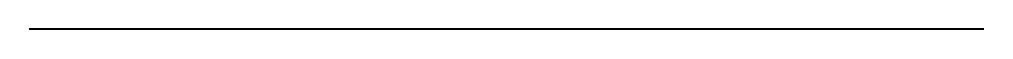
\begin{tikzpicture}[line width=1pt]
      \draw (0,0) -- (\textwidth,0);
    \end{tikzpicture}
    
    \vspace{3cm}
    {\LARGE \textbf{What's GraphQL}}

    \vspace{3cm}
    {\Large Activity 2: Distributed computing applications report}
    
    \vspace{3cm}
    
    \vfill
    {\Large \today}
    \vfill
    
    \vfill

    {\Large May Castells Raga \par}
    {\Large Anna Marin Nuño \par}
    \vfill
    
    \vspace{1cm}
    {\large Distributed Computing\\}
    {\large Grau en Enginyeria Informàtica\\}
    {\large Universitat de Lleida}
    
    \vspace{1cm}
    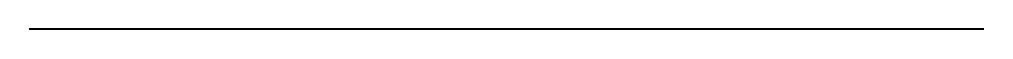
\begin{tikzpicture}[line width=1pt]
      \draw (0,0) -- (\textwidth,0);
    \end{tikzpicture}
  \end{center}
\end{titlepage}
\newpage

% Índice
%\renewcommand{\contentsname}{Índex}
\tableofcontents
\newpage

\section{Brief introduction}


In this project, we created a simple web service that uses four APIs to get information about animals and maps. The web service backend is built with FastAPI and the frontend with React. We started with a github simple template for FastAPI and React applications that the teacher showed us in class and then we added the required features and modified some behaviors to fit our needs.

\section{Login system}

The login system supports classic username/password (OAuth2) authentication with tokens as we did in class

\textbf{Frontend}: The login page collects user credentials and dispatches a Redux action (\texttt{login}). This calls an API function (\texttt{loginWithOauth}) that sends a POST request to \texttt{/login/oauth} with the username and password. If successful, the backend returns an \texttt{access\_token} and \texttt{refresh\_token}, which are stored in Redux state (\texttt{tokensSlice}).
  \item \textbf{Backend}: The \texttt{/login/oauth} endpoint (in \texttt{api/api_v1/endpoints/login.py}) authenticates the user using the provided credentials. If valid, it generates an access token (short-lived JWT) and a refresh token (long-lived JWT, also stored in the DB for revocation). The access token is used for authenticating API requests.
\end{itemize}

\section{The distl: ETL Providers for Animal Data}

The ``distl'' (Data Integration Service Layer) is the part of the backend responsible for gathering, normalizing, and storing animal observation data from multiple external sources. We used 4 different APIs: eBird for bird observations, Wildlife for image-based animal recognition, Ninjas for general animal data, and OpenStreetMaps and Photon for geospatial data, basicaly for geocoding and getting coordinates.

The distl is a set of ETL (Extract, Transform, Load) providers. Each provider is a Python class that knows how to fetch data from a specific source (like eBird, Wildlife, or OpenStreetMaps), clean it up, and save it in our database in a consistent format. For example, the EBirdProvider connects to the eBird API, downloads recent bird observations, and transforms them into our internal schema. The same pattern is followed for other sources, each with its own provider class.

The ETL process works like this: first, the provider fetches raw data from the external API. Then, it normalizes the data, this means converting all the different field names, types, and structures into a common format that is used. Finally, the provider saves both the raw and normalized data in MongoDB, so can always trace back where each observation came from.

Since all ETL looked pretty similar, we created a base abstract class called `ETLProvider` that defines the common interface and shared functionality for all providers. Each specific provider (like `EBirdProvider`, `WildlifeProvider`, etc.) extends this base class and implements the details for its own data source. This design pattern is shown in the following diagram:

\begin{figure}[H]
    \centering
    \includegraphics[width=0.8\textwidth]{uml_dstl.drawio.png}
    \caption{ETL Providers Design Pattern}
    \label{fig:etl_providers}
\end{figure}


\subsection{EBirdProvider}

The `EBirdProvider` extends `ETLProvider` and is responsible for importing bird data from the eBird API. It sets up API keys, URLs, and a logger in its constructor. The method `get_species_codes` looks up eBird species codes for a given common name, using a cached taxonomy. The `fetch` method downloads raw bird observation data, handling retries and deduplication. The `normalize` method converts eBird data into the internal schema, mapping fields like species, sci_name, lat, lon, date, location, how_many, and obs_id. There are also methods to save raw and normalized data (`save_raw_data`, `save_normalized_data`), and `get_observations` retrieves recent observations for a species from the database, using cache if available.

\subsection{WildlifeProvider}

The `WildlifeProvider` is for the Wildlife API. It sets up API keys and URLs in its constructor. The `fetch` method handles image preprocessing (resizing or compressing if needed)\footnote{Compressing is a key part because Wildlife API imagee limit size is 5MB and the total API usage is 1GB}, sends the image to the Wildlife API, and returns the response. The `normalize` method extracts and standardizes annotation data (id, label, confidence, taxonomy, bbox) from the API response.

\subsection{NinjasProvider}

The `NinjasProvider` is for the Ninjas API. It sets up API keys and URLs in its constructor. The `fetch` method queries the Ninjas API for animal data by name, tries fallback strategies if no results, and filters results. The `normalize` method converts the Ninjas API response into a list of dictionaries with name, taxonomy, locations, and characteristics. The `save` method saves both raw and normalized data to the database.

\subsection{OpenStreetMapsProvider}

The `OpenStreetMapsProvider` is for geospatial data. It sets up API keys and URLs in its constructor. The method `get_map_for_locations` takes a list of locations, queries Photon (an OSM geocoder), extracts coordinates, and returns them along with a computed center. The `fetch` method queries the Photon API for geocoding results, and `normalize` converts Photon/OSM data into a list of dictionaries with place_id, coordinates, and other properties.

All providers follow the same pattern: fetch data from their source, normalize it, and store it in MongoDB. Each provider handles the quirks and requirements of its own API, so the rest of the application can work with a unified data model.

\end{document}



